\section{Primul modul}

	Primul modul și cel mai important era cel de înregistrarea a cererilor de despăgubire.
	Am discutat despre soluția actuală, ce probleme are, ce câmpuri ar trebui să fie obligatorii și unde am putea optimiza interacțiunea clientului cu pagina web.

	\begin{figure}
		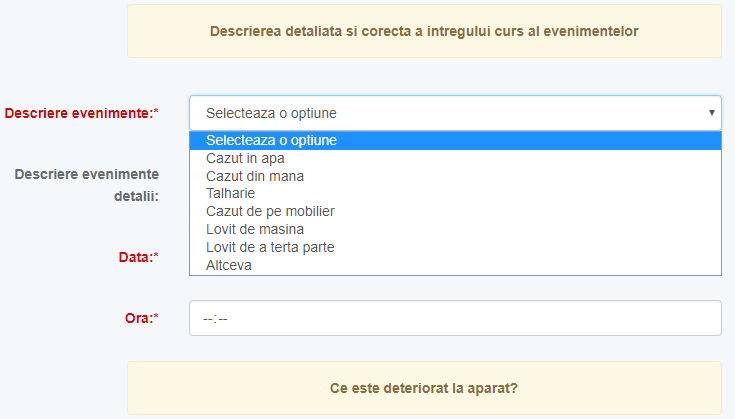
\includegraphics[width=\linewidth]{../imagini/descriere_eveniment.png}
		\caption{Descriere evenimente}
		\label{fig:descriere_evenimente}
	\end{figure}

	Un bun exemplu de modificări iterative asupra primului concept este la descrierea evenimentelor, după cum puteți observa în figura~\ref{fig:descriere_evenimente}.

	Inițial fusese vorba despre un simplu câmp text ce va fi la latitudinea utilizatorului spre a fi completat, dar mulțumită experienței în domeniu, cele mai des folosite motive au fost puse în schimb în această listă.
	În cazul în care s-a selectat „Altceva”, detaliile despre descrierea evenimentului devine obligatorie, pentru a ajuta clientul să identifice câmpurile ce trebuiesc completate.

	De asemenea, data și ora au un format ușor de înțeles și respectat, iar atunci când se selectează câmpul respectiv, apare un element vizual ajutător pentru a introduce corect data și ora.

	Pentru acest modul, trebuia să fie funcțională partea din spate de încărcare poze și gestionare a cererilor, dar și mai important, trebuia să fie gândită deja structura bazei de date, pentru modulele ulterioare.


	Secțiunea de rapoarte nu exista, dar puteai să cauți în sistemul de cereri în funcție de:
	\begin{itemize}
		\item Nume.
		\item Prenume.
		\item Număr de telefon.
		\item Numele aparatului.
		\item Email.
		\item Id-ul cererii de despăgubire.
	\end{itemize}
